\section{Specifying a Test Plan}

Following is a test plan for the \texttt{Velocity} class. 
It covers the intended behaviour of the class, the need for review, and testing objectives 
at the specification, implementation, and interaction levels.

\renewcommand{\arraystretch}{1.3}

\begin{longtable}{|p{4cm}|p{11cm}|}
\hline
\textbf{Plan Item} & \textbf{Description} \\
\hline
\endfirsthead

\hline
\textbf{Plan Item} & \textbf{Description} \\
\hline
\endhead

\hline
\endfoot

\hline
\endlastfoot

\textbf{Objectives for the class} &
The \texttt{Velocity} class must represent the motion of the puck using 
a non-negative scalar speed, a direction (in degrees), and corresponding 
horizontal and vertical components. These values must remain internally 
consistent at all times.

Specifically, the class should correctly construct a velocity from a 
given speed and direction, maintain consistency between \texttt{speed}, 
\texttt{speedX}, and \texttt{speedY}, and ensure that the direction 
determines the correct sign of each component (negative when moving 
left or down). In addition, bounce operations such as \texttt{reverse}, 
\texttt{reverseX}, and \texttt{reverseY} must update the velocity in a 
way that reflects expected physical behaviour. Getter methods must always 
return the current valid state. \\
\hline

\textbf{Inspection / review requirements} &
A design and code review is required prior to testing for several reasons:

\begin{enumerate}
\item Specification details are unclear. The informal description 
does not fully define how certain cases should be handled, such as 
direction values outside the range $0$-$359$, the behaviour of the 
default constructor, or whether angles like $360^\circ$ are equivalent 
to $0^\circ$. These ambiguities must be resolved before writing tests.

\item We want to ensure trigonometric and numerical correctness. The calculation 
of \texttt{speedX} and \texttt{speedY} depends on sine and cosine functions 
followed by conversion to integers. This introduces potential rounding and 
sign errors, especially at boundary angles such as $0^\circ$, $90^\circ$, 
$180^\circ$, and $270^\circ$.

\item We want to ensure the preservation of internal relationships. Any 
method that updates the velocity must maintain consistency between the 
scalar speed and its components. A review helps ensure that this 
relationship is re-established after every update.
\end{enumerate}

Without this review, test cases may reflect incorrect assumptions 
rather than actual intended behaviour. \\
\hline

\textbf{Specification-based testing objectives} &
When treating the class as a black box, the goal is to verify that each public method behaves according to its expected contract.

Testing should include:
\begin{itemize}
\item Typical cases. Representative speeds and directions across all four 
quadrants.
\item Boundary values. Directions such as $0$, $90$, $180$, $270$, and 
$359$, and speeds such as $0$ and large values.
\item Equivalence classes. Combinations of positive and negative values 
for \texttt{speedX} and \texttt{speedY}.
\item Invalid inputs (if applicable). For example, negative speeds or 
out-of-range directions.
\end{itemize}

Tests should confirm that outputs match expectations and that the observable behaviour of the class aligns with its specification. \\
\hline

\textbf{Implementation-based testing objectives} &
When treating the class as a white box, the goal is to exercise the internal logic and achieve strong structural coverage.

This includes:
\begin{itemize}
\item Statement and branch coverage, ensuring all methods and decision 
points are executed.
\item Condition coverage, testing how sign decisions are made based on 
direction.
\item Path coverage, particularly for direction normalization logic.
\item Rounding behaviour, verifying correctness near angles where integer 
rounding affects results ($45^\circ$, $135^\circ$, $225^\circ$, 
$315^\circ$).
\end{itemize}

These tests increase confidence that the implementation correctly handles all internal cases. \\
\hline

\textbf{Interaction-based testing objectives} &
The goal is to verify that sequences of method calls produce consistent and expected results, and that operations compose correctly.

Key interaction checks include:
\begin{itemize}
\item \texttt{setDirection} updates components without changing speed.
\item \texttt{setSpeed} rescales components while preserving direction.
\item Applying \texttt{reverseX} and \texttt{reverseY} together produces 
the same result as \texttt{reverse}.
\item Applying reverse operations twice returns the object to its original 
state.
\item Any sequence of updates followed by getters yields a state that 
remains internally consistent.
\end{itemize}

These tests ensure that method interactions do not violate expected 
behaviour over time. \\
\hline

\end{longtable}

\section{Contract-Based Specification}

Boolean expressions are defined in pseudocode. 
The notation \texttt{old(e)} refers to the value of an expression 
before execution. Directions are assumed to be in degrees and within 
the range $[0, 360)$.

\subsection*{Class Invariant}

\begin{verbatim}
invariant:
    speed >= 0
    && 0 <= direction < 360
    && speedX == round(speed * cos(direction))
    && speedY == round(speed * sin(direction))
    && abs(speedX) <= speed
    && abs(speedY) <= speed
    // sign constraints based on direction
    && (direction > 90 && direction < 270 ==> speedX <= 0)
    && (direction < 90 || direction > 270 ==> speedX >= 0)
    && (direction > 180 && direction < 360 ==> speedY <= 0)
    && (direction > 0 && direction < 180 ==> speedY >= 0)
\end{verbatim}

\subsection*{Constructors}

\textbf{Velocity()}

\textbf{Pre:} true

\textbf{Post:}
\begin{verbatim}
speed == 0
&& direction == 0
&& speedX == 0
&& speedY == 0
&& invariant holds
\end{verbatim}

\textbf{Velocity(Speed speed, Direction direction)}

\textbf{Pre:}
\begin{verbatim}
speed != null && direction != null
&& speed >= 0
&& 0 <= direction < 360
\end{verbatim}

\textbf{Post:}
\begin{verbatim}
this.speed == speed
&& this.direction == direction
&& this.speedX == round(speed * cos(direction))
&& this.speedY == round(speed * sin(direction))
&& invariant holds
\end{verbatim}

\subsection*{Getters}

\textbf{getSpeed()}

\textbf{Pre:} true

\textbf{Post:}
\begin{verbatim}
result == this.speed
&& result >= 0
&& object state remains unchanged
\end{verbatim}

\textbf{getSpeedX()}

\textbf{Pre:} true

\textbf{Post:}
\begin{verbatim}
result == this.speedX
&& abs(result) <= this.speed
&& object state remains unchanged
\end{verbatim}

\textbf{getSpeedY()}

\textbf{Pre:} true

\textbf{Post:}
\begin{verbatim}
result == this.speedY
&& abs(result) <= this.speed
&& object state remains unchanged
\end{verbatim}

\textbf{getDirection()}

\textbf{Pre:} true

\textbf{Post:}
\begin{verbatim}
result == this.direction
&& 0 <= result < 360
&& object state remains unchanged
\end{verbatim}

\subsection*{Setters}

\textbf{setSpeed(Speed speed)}

\textbf{Pre:}
\begin{verbatim}
speed != null && speed >= 0
\end{verbatim}

\textbf{Post:}
\begin{verbatim}
this.speed == speed
&& this.direction == old(this.direction)
&& this.speedX == round(speed * cos(this.direction))
&& this.speedY == round(speed * sin(this.direction))
&& invariant holds
\end{verbatim}

\textbf{setDirection(Direction direction)}

\textbf{Pre:}
\begin{verbatim}
direction != null && 0 <= direction < 360
\end{verbatim}

\textbf{Post:}
\begin{verbatim}
this.direction == direction
&& this.speed == old(this.speed)
&& this.speedX == round(this.speed * cos(direction))
&& this.speedY == round(this.speed * sin(direction))
&& invariant holds
\end{verbatim}

\subsection*{Direction Reversal Methods}

\textbf{reverse()}

\textbf{Pre:} true

\textbf{Post:}
\begin{verbatim}
this.speed == old(this.speed)
&& this.direction == (old(this.direction) + 180) mod 360
&& this.speedX == -old(this.speedX)
&& this.speedY == -old(this.speedY)
&& invariant holds
\end{verbatim}

\textbf{reverseX()}

\textbf{Pre:} true

\textbf{Post:}
\begin{verbatim}
this.speed == old(this.speed)
&& this.speedX == -old(this.speedX)
&& this.speedY == old(this.speedY)
&& this.direction == (540 - old(this.direction)) mod 360
&& invariant holds
\end{verbatim}

\textbf{reverseY()}

\textbf{Pre:} true

\textbf{Post:}
\begin{verbatim}
this.speed == old(this.speed)
&& this.speedY == -old(this.speedY)
&& this.speedX == old(this.speedX)
&& this.direction == (360 - old(this.direction)) mod 360
&& invariant holds
\end{verbatim}

\section{Test Cases}

Each test case specifies the input state, the operation performed, and the expected outcome.

\subsection*{setDirection}

\textbf{Test 1: updating direction preserves speed and updates components}

\textbf{Input:}  
Initial state: $v = \text{new Velocity}(10, 0)$  
Call: $v.\text{setDirection}(90)$  

\textbf{Expected Output:}
\begin{verbatim}
v.getDirection() == 90
v.getSpeed() == 10
v.getSpeedX() == 0
v.getSpeedY() == 10
class invariant holds
\end{verbatim}

\subsection*{setSpeed}

\textbf{Test 1: updating speed preserves direction and rescales components}

\textbf{Input:}  
Initial state: $v = \text{new Velocity}(5, 180)$  
Call: $v.\text{setSpeed}(20)$  

\textbf{Expected Output:}
\begin{verbatim}
v.getSpeed() == 20
v.getDirection() == 180
v.getSpeedX() == -20
v.getSpeedY() == 0
class invariant holds
\end{verbatim}

\subsection*{reverse}

\textbf{Test 1: reversing motion from right to left}

\textbf{Input:}  
$v = \text{new Velocity}(10, 0)$  
Call: $v.\text{reverse}()$

\textbf{Expected Output:}
\begin{verbatim}
direction == 180
speedX == -10
speedY == 0
speed == 10
\end{verbatim}

\textbf{Test 2: reversing from northeast to southwest}

\textbf{Input:}  
$v = \text{new Velocity}(14, 45)$  
Call: $v.\text{reverse}()$

\textbf{Expected Output:}
\begin{verbatim}
direction == 225
speedX == -10
speedY == -10
speed == 14
\end{verbatim} 

\textbf{Test 3: applying reverse twice restores original state}

\textbf{Input:}  
$v = \text{new Velocity}(8, 123)$  
Call: $v.\text{reverse}()$ twice

\textbf{Expected Output:}
\begin{verbatim}
Final (speed, direction, speedX, speedY)
matches the original state
\end{verbatim}

\textbf{Test 4: reversing straight downward motion}

\textbf{Input:}  
$v = \text{new Velocity}(7, 270)$  
Call: $v.\text{reverse}()$

\textbf{Expected Output:}
\begin{verbatim}
direction == 90
speedX == 0
speedY == 7
speed == 7
\end{verbatim}

\textbf{Test 5: reversing when speed is zero}

\textbf{Input:}  
$v = \text{new Velocity}(0, 60)$  
Call: $v.\text{reverse}()$

\textbf{Expected Output:}
\begin{verbatim}
direction == 240
speedX == 0
speedY == 0
speed == 0
\end{verbatim}

\subsection*{reverseX}

\textbf{Test 1: bounce off vertical wall while moving right}

\textbf{Input:}  
$v = \text{new Velocity}(10, 0)$  
Call: $v.\text{reverseX}()$

\textbf{Expected Output:}
\begin{verbatim}
speedX == -10
speedY == 0
direction == 180
speed == 10
\end{verbatim}

\textbf{Test 2: northeast becomes northwest}

\textbf{Input:}  
$v_1 = \text{new Velocity}(14, 45)$  
$v_2 = \text{new Velocity}(14, 45)$  
Call: $v_1.\text{reverseX}()$

\textbf{Expected Output:}
\begin{verbatim}
v_1.direction == 135
v_1.speedX == -v_2.speedX
v_1.speedY == v_2.speedY
speed == 14
\end{verbatim}

\textbf{Test 3: vertical motion remains unchanged}

\textbf{Input:}  
$v = \text{new Velocity}(10, 90)$  
Call: $v.\text{reverseX}()$

\textbf{Expected Output:}
\begin{verbatim}
speedX == 0
speedY == 10
direction == 90
speed == 10
\end{verbatim}

\textbf{Test 4: applying reverseX twice restores original state}

\textbf{Input:}  
$v = \text{new Velocity}(12, 200)$  
Call: $v.\text{reverseX}()$ twice

\textbf{Expected Output:}
\begin{verbatim}
Final state identical to initial state
(speed, direction, speedX, speedY)
\end{verbatim}

\textbf{Test 5: reverseX followed by reverseY equals reverse}

\textbf{Input:}  
$a = \text{new Velocity}(10, 30)$  
$b = \text{new Velocity}(10, 30)$  

Call:  
$a.\text{reverseX}();\ a.\text{reverseY}();$  
$b.\text{reverse}();$

\textbf{Expected Output:}
\begin{verbatim}
a.speed == b.speed
a.direction == b.direction
a.speedX == b.speedX
a.speedY == b.speedY
\end{verbatim}

\section{Test Automation}
Please see the associated GitHub repository for the test suite. I've
used Playwright as that is the tool I am most familiar with.

\subsection*{a)}

I selected \texttt{checkboxes} and \texttt{dropdown} as the two cases from 
the provided list. The tests are provided in \texttt{test\_checkboxes.py} 
and \texttt{test\_dropdown.py}, respectively.

\medskip

\subsubsection*{Checkboxes (\url{https://the-internet.herokuapp.com/checkboxes})}

This page contains two checkboxes with predefined initial states and supports 
basic user interactions (checking and unchecking). The test suite verifies both 
the default configuration and the correctness of state transitions under user actions.

\medskip

Initial state, \texttt{test\_initial\_checkbox\_states()}: 
Verifies that the first checkbox is initially unchecked and the second is checked, 
ensuring the page loads with the expected default configuration.

\medskip

Check action, \texttt{test\_check\_first\_checkbox()}:
Checks that selecting an unchecked checkbox correctly updates its state to checked, 
confirming basic interaction behaviour.

\medskip

Uncheck action, \texttt{test\_uncheck\_second\_checkbox()}: 
Verifies that an initially checked checkbox can be unchecked, ensuring that state 
changes in both directions are supported.

\medskip

Toggle consistency, \texttt{test\_toggle\_twice\_returns\_original()}:
Checks that performing a check followed by an uncheck returns the checkbox to its 
original state, validating stability under repeated operations.

\medskip

Multiple selection, \texttt{test\_both\_checkboxes\_checked()}:  
Ensures that both checkboxes can be selected simultaneously, confirming that 
independent elements do not interfere with each other.

\medskip

\subsubsection*{Dropdown (\url{https://the-internet.herokuapp.com/dropdown})}

This page contains a dropdown menu with a placeholder and two selectable options. 
The tests verify correct selection behaviour and consistency of the selected value.

\medskip

Default state, \texttt{test\_default\_dropdown\_state()}: 
Verifies that no option is selected by default (placeholder is active), ensuring 
correct initialization of the dropdown.

\medskip

Select first option, \texttt{test\_select\_first\_option()}:
Checks that selecting the first option updates the dropdown value correctly.

\medskip

Select second option, \texttt{test\_select\_second\_option()}:
Verifies correct behaviour when selecting the second option.

\medskip

Switching options, \texttt{test\_switch\_between\_options()}:
Ensures that changing the selection from one option to another updates the state 
accordingly, validating transitions between valid inputs.

\medskip

Idempotence, \texttt{test\_reselect\_same\_option()}:
Checks that selecting the same option multiple times does not produce unexpected 
behaviour and the state remains consistent.

The website passes all of the above tests.

\begin{center}
    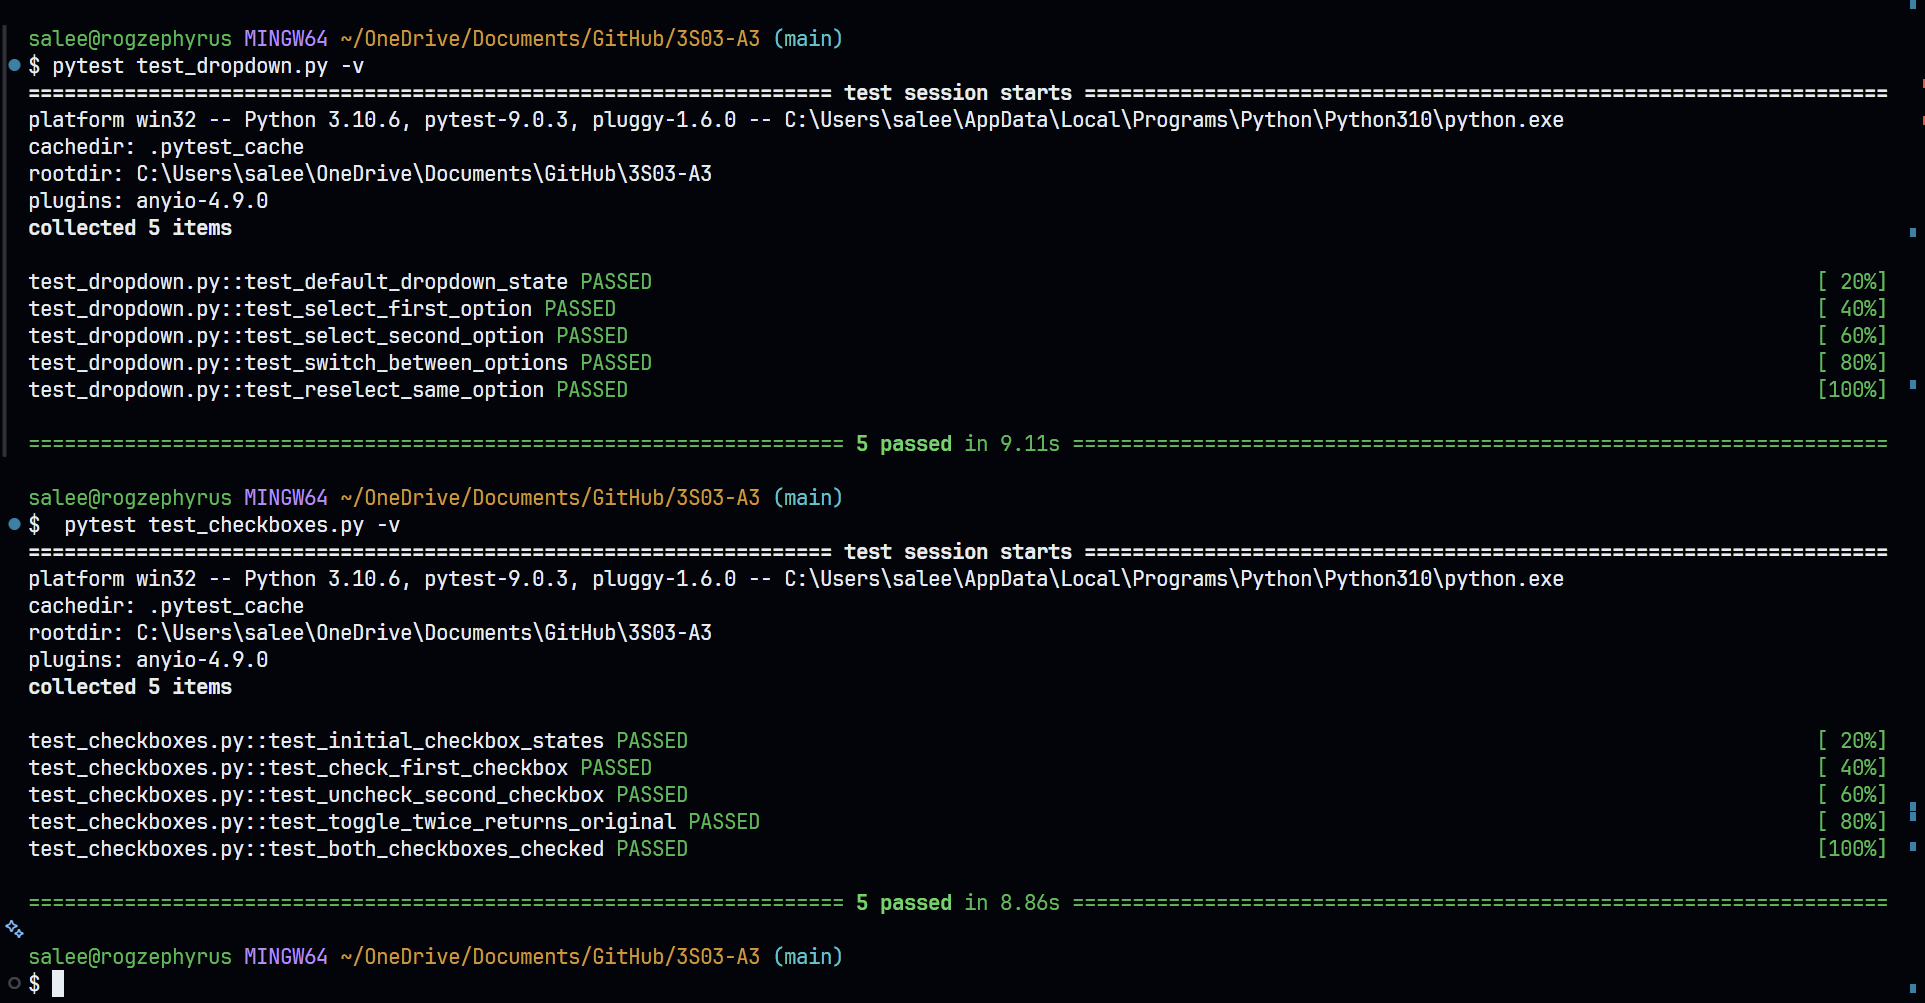
\includegraphics[width=1\textwidth]{../4a_tests_pass.png}
\end{center}

\subsection*{b)}
The tests are provided in \texttt{test\_saucedemo.py}. An activity
diagram for this process is shown below. Apologies for the image
quality as the diagram is kind of long, I have also attached
an svg of the same diagram in the GitHub repo in case this one is difficult
to read.

\begin{center}
    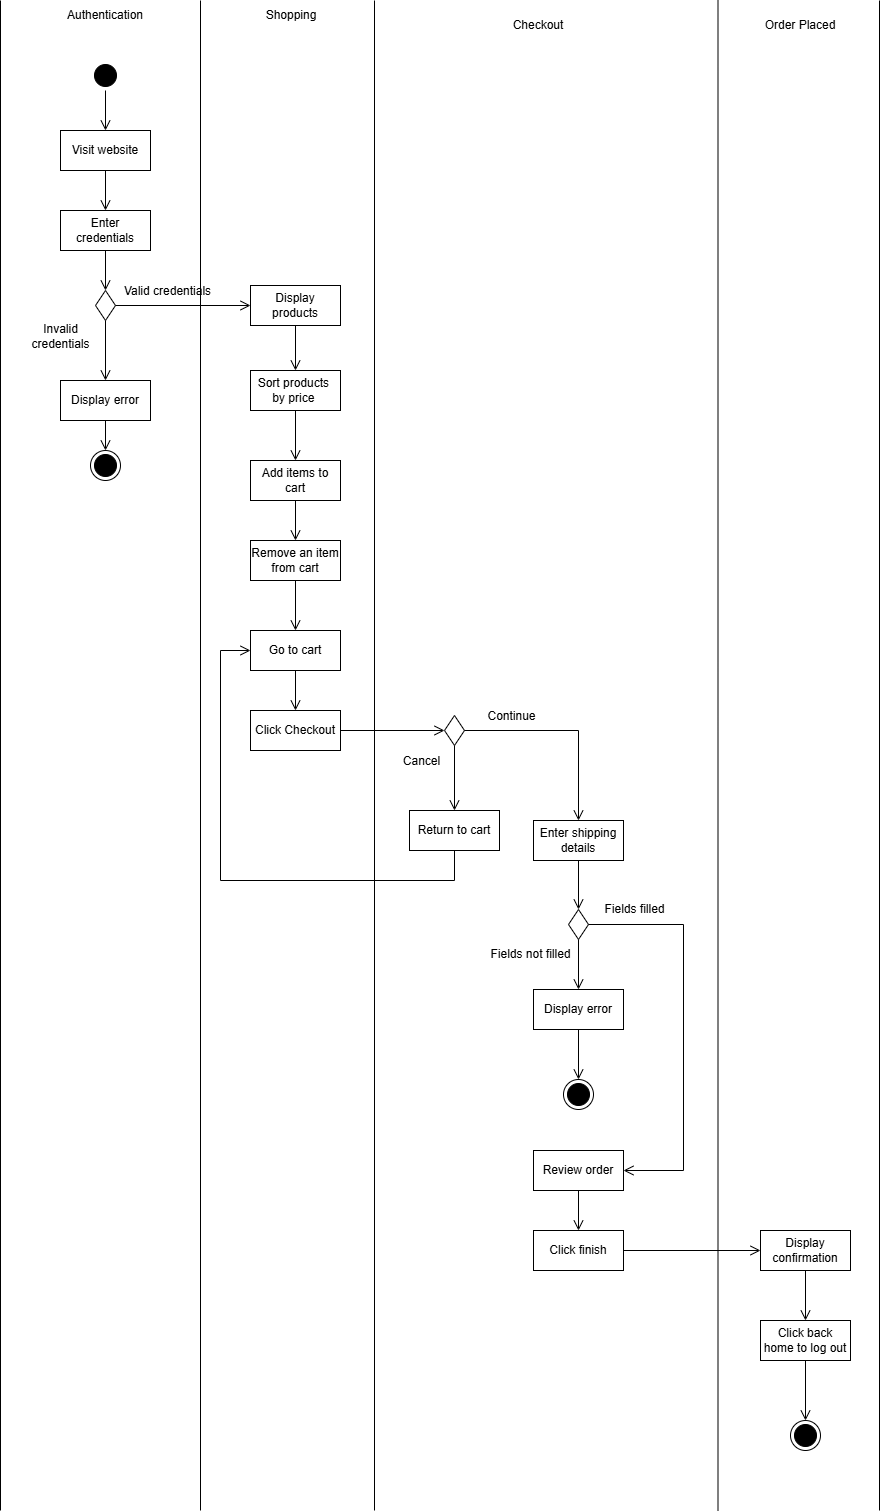
\includegraphics[width=0.8\textwidth]{../Q4b.png}
\end{center}

\subsection*{Rationale}

I first mapped out the user flow using an activity diagram, splitting it 
into four main parts: authentication, shopping, checkout, and order placed. 
This made it easier to see where the system branches (like valid vs invalid 
login, cancel vs continue at checkout, and whether required fields are filled 
or not).

The main test (\texttt{test\_complete\_purchase\_flow}) follows the full happy 
path. This includes logging in successfully, viewing and sorting products, 
adding and removing items, going through checkout, verifying totals, and 
finishing the order. This test basically ensures the core functionality works 
end-to-end.

To cover the important branches in the diagram, I added a few smaller targeted 
tests:
\begin{itemize}
    \item \texttt{test\_invalid\_user\_displays\_error}: checks the invalid 
    login case.
    \item \texttt{test\_checkout\_with\_missing\_fields\_displays\_error}: 
    checks that the form validation triggers when required fields are missing.
    \item \texttt{test\_cancel\_checkout\_returns\_to\_cart}: checks that 
    cancelling checkout correctly returns the user to the cart.
\end{itemize}

So overall, each decision point in the diagram is covered at least once. The 
happy path handles all the “successful” transitions, and the extra tests cover 
the main failure/alternative paths.

I didn't try to test every possible invalid input (like every missing field 
combination or all bad credential cases), since those would mostly hit the same 
validation logic and wouldn't add much value. Instead, I focused on cases that 
actually represent different behaviours in the system.

I also included a more meaningful check during checkout (verifying that 
subtotal + tax equals the total), so it's not just clicking through pages. 
Finally, using Playwright's \texttt{expect()} helps avoid flaky tests since 
it waits for the UI state instead of relying on timing.


